\documentclass[10pt]{article}
\usepackage[dutch]{babel}
\usepackage{todonotes}
\usepackage{amssymb}
\usepackage{amsmath}
% \usepackage[parfill]{parskip}
\usepackage{pgffor}
\usepackage{graphicx}
\usepackage{subcaption}
\usepackage{xltabular}
\usepackage{float}
\usepackage{enumitem}
\usepackage{hyperref}
\usepackage{rest-api}
\usepackage[margin=3.5cm]{geometry}

\setlist[itemize]{leftmargin=*}
\setlength{\parskip}{1em}

\makeatletter
\renewcommand{\rmdefault}{\sfdefault}
\def\subtitle#1{\gdef\@subtitle{#1}}

\def\leftHeader#1{\listadd\@leftHeader{#1}}
\def\rightHeader#1{\listadd\@rightHeader{#1}}

\def\@maketitle{
\renewcommand{\do}[1]{##1

}
\begin{minipage}[t]{5cm}
\flushleft
\dolistloop{\@leftHeader}
\end{minipage}
\hfill
\begin{minipage}[t]{5cm}
\flushright
\dolistloop{\@rightHeader}
\end{minipage}
\centering

\vspace{7cm}
% \vfill
{\huge\bfseries\@title\par}
\vfill
% \vspace{1cm}
\thispagestyle{empty}
\clearpage
}
\makeatother

\title{Verslag

\Large Project Gedistribueerde Systemen}

\leftHeader{Ward Gauderis}
\leftHeader{20183431}
\rightHeader{Gedistribueerde Systemen}
\rightHeader{Informatica}
\rightHeader{UAntwerpen}
\leftHeader{10/01/2021}

\begin{document}
\maketitle

\vfill
\tableofcontents
\vfill
\clearpage

\section{Praktisch}
De webapplicatie is opgesplitst in verschillende Docker containers die beheerd worden met Docker-Compose. Enkel het docker-compose commando, een draaiende Docker daemon en Docker gebruikersrechten zijn noodzakelijk om de applicatie op te starten. Hiervoor zijn de scriptjes \textbf{install.sh} en \textbf{run.sh} voorzien.
Binnen de containers zelf worden automatisch de verschillende dependencies geïnstalleerd.

\noindent Zowel de API als de bijhorende site zijn beschikbaar op poort 80 van \textbf{localhost}.
De applicatie is geïnitialiseerd met de data die werd voorzien via Blackboard.
Gebruikers van de applicatie vallen in 5 categorieën (combinaties zijn mogelijk) met verschillende rechten. Voor elk van deze gebruikers is er een account aangemaakt waarmee de applicatie kan getest worden.

\begin{xltabular}{\linewidth}{|l|l|l|}
	\hline
	\textbf{Gebruikersrol} & \textbf{Username} & \textbf{Password}\\
	\hline
	Anonieme gebruiker &&\\
	\hline
	Geregistreerde gebruiker & Voetbalfan & Voetbalfan\\
	\hline
	Geregistreerde gebruiker gelinkt aan een team & Voetballer & Voetballer\\
	\hline
	Administator & Admin & Admin\\
	\hline
	Superadministrator & Super & Super\\
	\hline
\end{xltabular}

\clearpage
\section{Tools}

Wat betreft de tools heb ik me gehouden aan de lijst van de opdracht, met enkele aanpassingen en toevoegingen.\\
In plaats van Bootstrap, gebruik ik Bulma als CSS framework. In het Programming Project Databases van vorig jaar gebruikten we exact dezelfde technologieën als in dit project en toen hadden we voornamelijk spijt van het feit dat we Bootstrap hadden gebruikt omwille van de verborgen complexiteit. Bulma is een meer light-weight variant hierop zonder javascript.\\
Eveneens gebruik ik voor de geocoding niet de Google Geocoding API maar Positionstack omdat deze service minder persoonlijke data van mij opvroeg om een gratis account aan te maken.\\
Verder maak ik gebruik van JSON Web Tokens voor de token-based authentication bij de API, van Flask-Login voor de session based authentication bij de website frontend, van WTForms om enkele aspecten van de HTML-forms te vereenvoudigen, van de webserver Nginx als reverse proxy die het verkeer tussen de verschillende Docker containers en de gebruiker orkestreert en van Gunicorn als WSGI application server om de communicatie tussen Nginx en Flask te overzien.

\clearpage
\section{Design}
De applicatie heb ik opgesplitst in 6 verschillende containers op basis van functionaliteit die voorzien wordt en de rechten die nodig zijn om deze functionaliteit te mogen gebruiken.\\
Het is altijd mogelijk om de backend (vooral de API bestaande uit \textbf{Stats} en \textbf{CRUD}) verder op te splitsen in meer microservices, maar dit leek me vooral meer werk met zich mee te brengen en niet veel directe voordelen.

\begin{figure}[H]
	\centerline{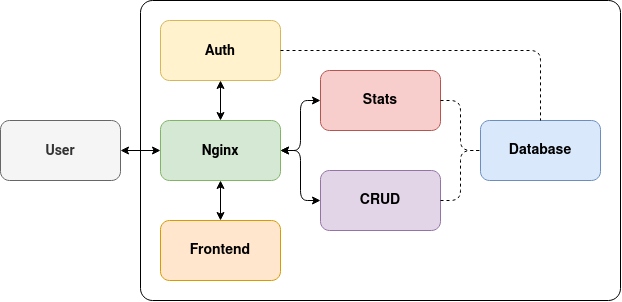
\includegraphics[width=\linewidth]{diagram}}
\end{figure}

\noindent Hier volgt een beschrijving per container.

\subsection{Nginx}
De \textbf{Nginx} container regelt het verkeer tussen de verschillende containers en zorgt ervoor dat de applicatie voor de gebruiker er als één geheel uitziet. De gebruiker heeft enkel toegang tot poort 80 van localhost terwijl alle interne HTTP-verkeer via poorten 5000 gaat. \textbf{Nginx} bepaalt welke requests naar welke microservice moeten worden doorgestuurd. Eveneens worden voor de API requests die autorisatie nodig hebben autorisatierequests gestuurd naar \textbf{Auth} vooraleer deze requests te forwarden.

\subsection{Auth}
De \textbf{Auth} service is een Flask applicatie die instaat voor de token-based authenticatie en de autorisatie van de API. Deze maakt gebruik van JSON web tokens die de gebruiker van de API moet voorzien in de autorisatieheader van zijn request. De service genereert JWT tokens op aanvraag van gebruikers met correcte HTTP basic access authentication.
Daarnaast autoriseert de \textbf{Auth} service ook gebruikers voor toegang tot bepaalde delen van de API door te antwoorden op autorisatierequests van \textbf{Nginx}.

\subsection{Stats}
De \textbf{Stats} service vormt samen met \textbf{CRUD} en \textbf{Auth} de van buitenaf toegankelijke API. Deze Flask applicatie staat in voor alle functionaliteit die toegankelijk is voor alle gebruikers en die geen autorisatie vereist. Deze container communiceert met de \textbf{Database} om alle vereiste statistieken uit de opdracht te voorzien, waaronder het genereren van de league tables, het oplijsten van bepaalde fixtures, het berekenen van de beste teams en het berekenen van statistieken omtrent een team of fixture. Deze service is eveneens verantwoordelijk voor het voorzien van weerdata voor toekomstige wedstrijden en interageert dus met de OpenWeatherMap en Positionstack API.
\subsection{CRUD}
De \textbf{CRUD} service staat in voor alle functionaliteit van de API die niet voor alle gebruikers toegankelijk is. Requests hiernaar moeten geautoriseerd worden door de \textbf{Auth} service. Zoals de naam aangeeft, is deze service dan ook voornamelijk verantwoordelijk voor de create, read, update en delete operaties op de verschillende entiteiten in de \textbf{Database}. Het grootste deel van deze operaties is enkel toegestaan voor admins en superadmins, maar zoals de opdracht aangeeft, moeten teamleden bijvoorbeeld ook toegang krijgen tot hun clubinformatie en scores. Eveneens zijn sommige readoperaties ook toegestaan voor alle gebruikers indien deze enkel publiek toegankelijke data opvragen. Net zoals bij alle API functionaliteit worden deze operaties sterk gecontroleerd op inconsistenties om interne databasefouten te vermijden.
\subsection{Database}
De \textbf{Database} container is een PostgreSQL server waarmee andere containers kunnen communiceren via poort 5432. Dit gebeurt langs hun kant via SQLAlchemy. De database is geïnitialiseerd met alle voorziene data plus vier gebruikers om te testen. Een groot deel van de design van de database werd bepaald door de structuur van deze voorziene data. Buiten de 5 entiteiten uit de opdracht, bevat de database ook nog een tabel voor de divisies. Seizoenen werden hierin niet opgenomen maar worden afgeleid uit de de matchdata om inconsistenties te vermijden. Verschillende constraints zijn aanwezig op de tabellen om de integriteit van de database te behouden.

\subsection{Frontend}
De \textbf{Frontend} service is een Flask applicatie die voor de gebruiker ervan communiceert met de achterliggende API. Deze service heeft dus geen speciale interne connecties met bv.\ de database en zou evengoed extern kunnen opereren of geschreven zijn door een gebruiker zelf. De \textbf{Frontend} voorziet een (Bulma) GUI voor alle API operaties, gecombineerd in een overzichtelijke website. Zo wordt de token-based login vertaald naar een session-based login en worden create, update en delete requests omgezet in HTML forms. Meldingen over incorrecte operaties uit de backend worden eveneens doorgepropageerd naar de frontend zodat de gebruiker weet wat hij verkeerd doet.
Voor alle vereiste functionaliteit uit de opdracht is een pagina voorzien. Pagina's die enkel toegankelijk zijn voor gebruikers met bepaalde rechten worden verborgen voor andere gebruikers om verwarring te vermijden.

\clearpage
\section{API}
De van buitenaf aanspreekbare API is verspreid over de \textbf{Auth}, \textbf{Stats} en \textbf{CRUD} microservices en is beschikbaar via poort 80 op localhost/api. Als RESTful API wordt er gebruik gemaakt van de verschillende HTTP request methods en het json-formaat om duidelijker te zijn over het doel van de request. Hier volgt een beschrijving van alle aanspreekbare API endpoints.

\noindent Indien de status code van de response niet gelijk is aan 200, zal het bericht steeds de volgende vorm hebben:

\vspace{2em}
\begin{routeResponseItemBody}
{ 
	"code" : <status code>,
	"description" : <description>,
	"error" : <status message>
}
\end{routeResponseItemBody}

\noindent Velden die optioneel zijn, kunnen zowel in de body van de request als de response worden weggelaten en defaulten naar null. Indien vereiste velden missen in requests, wordt dit gemeld. Om de beschrijvingen van de API endpoints wat in te korten, geef ik hier al de JSON representatie van de verschillende entiteiten in de database.


Club
\vspace{2em}
\begin{routeResponseItemBody}
{ 
	"stam_number": <club stam number>,
	"name": <club name>,
	"address": <club address>,
	"zip_code": <club zip code>,
	"city": <club city>,
	"website": <optional club website>
}
\end{routeResponseItemBody}

Team
\vspace{2em}
\begin{routeResponseItemBody}
{ 
	"id" : <team id>,
	"stam_number": <club stam number>,
	"suffix": <optional team suffix>,
	"colors": <team colors>,
	"name": <full team name>
}
\end{routeResponseItemBody}

Division
\vspace{2em}
\begin{routeResponseItemBody}
{ 
	"id" : <division id>,
	"name" : <division name>
}
\end{routeResponseItemBody}

Match
\vspace{2em}
\begin{routeResponseItemBody}
{ 
	"id" : <match id>,
	"division_id" : <division id>,
	"matchweek" : <match week>,
	"date" : <match date>,
	"time" : <match time>,
	"home_team_id" : <team id>,
	"away_team_id" : <team id>,
	"goals_home_team" : <optional home team goals>,
	"goals_away_team" : <optional away team goals>,
	"status" : <optional status (Postponed, Canceled, Forfait)>,
	"referee_id" : <optional referee id>,
	"home_team_name" : <team name>,
	"away_team_name" : <team name>,
	"division_name" : <division name>,
	"referee_name" : <optional referee name>,
	"season" : <match season (bv. 2020 voor 2020-2021)>
}
\end{routeResponseItemBody}

Referee
\vspace{2em}
\begin{routeResponseItemBody}
{ 
	"id" : <referee id>,
	"first_name" : <referee first name>,
	"last_name" : <referee last name>,
	"address" : <referee address>,
	"zip_code" : <referee zip_code>,
	"city" : <referee city>,
	"phone_number" : <referee phone number>,
	"email" : <referee email>,
	"date_of_birth" : <referee date of birth>
}
\end{routeResponseItemBody}

User
\vspace{2em}
\begin{routeResponseItemBody}
{ 
	"id" : <user id>,
	"username" : <username>,
	"email" : <email>,
	"team_id" : <optional team id>,
	"is_admin" : <bool>,
	"is_super_admin" : <bool>
	"team_name": <optional team name>,
	"stam_number": <optional club stam number>
}
\end{routeResponseItemBody}

\clearpage
\subsection{Auth}

\vspace{2em}

\begin{apiRoute}{post}{/api/auth}{Vraag JWT authenticatie token aan met HTTP basic access authentication.}
 Authorization: Basic <username:password in b64>
	\begin{routeResponse}{application/json}
		\begin{routeResponseItem}{200}{ok}
			\begin{routeResponseItemBody}
{ 
	"token" : <token>
}
			\end{routeResponseItemBody}
		\end{routeResponseItem}
	\end{routeResponse}
\end{apiRoute}

\subsection{Stats}

Deze endpoints vereisen geen authenticatie.

\vspace{1em}

\begin{apiRoute}{get}{/api/stats/league\_tables/<div>/<season>}{Vraag de league table op voor een bepaalde divisie en seizoen.}
	\begin{routeParameter}
		\routeParamItem{div}{divisie id of 0 voor alle}
		\routeParamItem{season}{seizoen (bv. 2020 voor seizoen 2020-2021) of 0 voor altijd}
	\end{routeParameter}

	\begin{routeResponse}{application/json}
		\begin{routeResponseItem}{200}{ok}
			\begin{routeResponseItemBody}
[{
	"GA": <goals against>,
	"GD": <goal difference>,
	"GF": <goals for>,
	"drawn": <matches drawn>,
	"lost": <matches lost>,
	"played": <matches played>,
	"points": <points>,
	"pos": <position>,
	"team": <TEAM>
	"won": <matches won>
}, ...]
			\end{routeResponseItemBody}
		\end{routeResponseItem}
	\end{routeResponse}
\end{apiRoute}

\begin{apiRoute}{get}{/api/stats/fixtures/<div>/<team>/<season>}{Vraag de fixtures op voor een bepaalde divisie, team en seizoen.}
	\begin{routeParameter}
		\routeParamItem{div}{divisie id of 0 voor alle}
		\routeParamItem{team}{team id of 0 voor alle}
		\routeParamItem{season}{seizoen (bv. 2020 voor seizoen 2020-2021) of 0 voor toekomstig}
	\end{routeParameter}

	\begin{routeResponse}{application/json}
		\begin{routeResponseItem}{200}{ok}
			\begin{routeResponseItemBody}
[
	<MATCH>, ...
]
			\end{routeResponseItemBody}
		\end{routeResponseItem}
	\end{routeResponse}
\end{apiRoute}

\begin{apiRoute}{get}{/api/stats/top/<season>}{Vraag de teams met de beste attack, defense en clean sheets op per divisie voor een bepaald seizoen.}
	\begin{routeParameter}
		\routeParamItem{season}{seizoen (bv. 2020 vor seizoen 2020-2021) of 0 voor alle}
	\end{routeParameter}

	\begin{routeResponse}{application/json}
		\begin{routeResponseItem}{200}{ok}
			\begin{routeResponseItemBody}
[{
	"best_attack": {
		"GF": <goals for>,
		<TEAM>
	},
	"best_defence": {
		"GA": <goals against>,
		<TEAM>
	},
	"most_clean_sheets": {
		"count": <clean sheet count>,
		<TEAM>
	},
	<DIVISION>
}, ...]
			\end{routeResponseItemBody}
		\end{routeResponseItem}
	\end{routeResponse}
\end{apiRoute}

\begin{apiRoute}{get}{/api/stats/fixtures/<id>}{Vraag informatie op omtrent een fixture.}
	\begin{routeParameter}
		\routeParamItem{id}{match id}
	\end{routeParameter}
,
	\begin{routeResponse}{application/json}
		\begin{routeResponseItem}{200}{ok}
			\begin{routeResponseItemBody}
{
	<MATCH>
	"location": <home team club location>,

	# enkel bij toekomstig fixtures
	"previous_games": <amount of games against each other>,
	"home_team_wins": <amount of games home team won against each other>,
	"away_team_wins": <amount of games away team won against each other>,
	"recent_matches": [

		<MATCH>, ...
	],
	"recent_matches_home_team": [{
		"id": <match id>,
		"result": <W/L/D>
	}, ...],
	"recent_matches_away_team": [{
		"id": <match id>,
		"result": <W/L/D>
	}, ...]

	# enkel voor matches komende week
	# is een errormelding als de weer/geolocation services niet correct reageren
	"weather": {
		"temp_max": <maximum temperature>,
		"temp_min": <minimum temperature>,
		"description": <description>,
		"icon": <icon id>,
		"humidity": <humidity percentage>,
		"feels_like": <feels like temperature>
	}
}
			\end{routeResponseItemBody}
		\end{routeResponseItem}
	\end{routeResponse}
\end{apiRoute}

\begin{apiRoute}{get}{/api/stats/teams/id}{Vraag informatie op omtrent een team.}
	\begin{routeParameter}
		\routeParamItem{id}{team id}
	\end{routeParameter}

	\begin{routeResponse}{application/json}
		\begin{routeResponseItem}{200}{ok}
			\begin{routeResponseItemBody}
[{
	<TEAM>,
	"recent_matches": [
		<MATCH>, ...
	],
	"future_matches": [
		<MATCH>, ...
	],
	"club": <CLUB>
}, ...]
			\end{routeResponseItemBody}
		\end{routeResponseItem}
	\end{routeResponse}
\end{apiRoute}

\subsection{CRUD}

Bij alle PUT operaties zijn de velden optioneel, deze velden worden niet aangepast in de database.

\subsubsection{Club}

\begin{apiRoute}{get}{/api/crud/clubs}{Verkrijg alle clubs.}
	\begin{routeResponse}{application/json}
		\begin{routeResponseItem}{200}{ok}
			\begin{routeResponseItemBody}
[
	<CLUB>, ...
]
\end{routeResponseItemBody}
		\end{routeResponseItem}
	\end{routeResponse}
\end{apiRoute}

\begin{apiRoute}{post}{/api/crud/clubs}{Creëer club.}
 Authorization: Bearer <token van admin of superadmin>
	\begin{routeRequest}{application/json}
		\begin{routeRequestBody}
<CLUB zonder stam_number>
		\end{routeRequestBody}
	\end{routeRequest}

	\begin{routeResponse}{application/json}
		\begin{routeResponseItem}{200}{ok}
			\begin{routeResponseItemBody}
{
	"stam_number": <club stam number>
}
			\end{routeResponseItemBody}
		\end{routeResponseItem}
	\end{routeResponse}
\end{apiRoute}

\begin{apiRoute}{get}{/api/crud/clubs/<stam\_number>}{Verkrijg club informatie.}
	\begin{routeParameter}
		\routeParamItem{stam\_number}{club stam number}
	\end{routeParameter}

	\begin{routeResponse}{application/json}
		\begin{routeResponseItem}{200}{ok}
			\begin{routeResponseItemBody}
<CLUB>
			\end{routeResponseItemBody}
		\end{routeResponseItem}
	\end{routeResponse}
\end{apiRoute}

\begin{apiRoute}{delete}{/api/crud/clubs/<stam\_number>}{Verwijder club.}
 Authorization: Bearer <token van admin of superadmin>
	\begin{routeParameter}
		\routeParamItem{stam\_number}{club stam number}
	\end{routeParameter}

	\begin{routeResponse}{application/json}
		\begin{routeResponseItem}{200}{ok}
			\begin{routeResponseItemBody}
			\end{routeResponseItemBody}
		\end{routeResponseItem}
	\end{routeResponse}
\end{apiRoute}


\begin{apiRoute}{put}{/api/crud/clubs/<stam\_number>}{Verander club informatie.}
 Authorization: Bearer <token van admin of superadmin of van een user gelinkt aan een team van deze club>
	\begin{routeParameter}
		\routeParamItem{stam\_number}{club stam number}
	\end{routeParameter}

	\begin{routeRequest}{application/json}
		\begin{routeRequestBody}
<CLUB zonder stam_number>
		\end{routeRequestBody}
	\end{routeRequest}

	\begin{routeResponse}{application/json}
		\begin{routeResponseItem}{200}{ok}
			\begin{routeResponseItemBody}
			\end{routeResponseItemBody}
		\end{routeResponseItem}
	\end{routeResponse}
\end{apiRoute}

%%%%%%%%%%%%%%%%%%%%%%%%%%%%%%%%%%%%%%%%%%%%%%%%%%%%%%%%%%%%%%%%%%%%%%%%%%%%%%%%%%%%%%%%%%%%%%%%%%%%%
\subsubsection{Team}

\begin{apiRoute}{get}{/api/crud/teams}{Verkrijg alle teams.}
	\begin{routeResponse}{application/json}
		\begin{routeResponseItem}{200}{ok}
			\begin{routeResponseItemBody}
[
	<TEAM>, ...
]
\end{routeResponseItemBody}
		\end{routeResponseItem}
	\end{routeResponse}
\end{apiRoute}

\begin{apiRoute}{post}{/api/crud/teams}{Creëer team.}
 Authorization: Bearer <token van admin of superadmin>
	\begin{routeRequest}{application/json}
		\begin{routeRequestBody}
<TEAM zonder id en name>
		\end{routeRequestBody}
	\end{routeRequest}

	\begin{routeResponse}{application/json}
		\begin{routeResponseItem}{200}{ok}
			\begin{routeResponseItemBody}
{
	"id": <team id>
}
			\end{routeResponseItemBody}
		\end{routeResponseItem}
	\end{routeResponse}
\end{apiRoute}

\begin{apiRoute}{get}{/api/crud/teams/<id>}{Verkrijg team informatie.}
	\begin{routeParameter}
		\routeParamItem{id}{team id}
	\end{routeParameter}

	\begin{routeResponse}{application/json}
		\begin{routeResponseItem}{200}{ok}
			\begin{routeResponseItemBody}
<TEAM>
			\end{routeResponseItemBody}
		\end{routeResponseItem}
	\end{routeResponse}
\end{apiRoute}

\begin{apiRoute}{delete}{/api/crud/teams/<id>}{Verwijder team.}
 Authorization: Bearer <token van admin of superadmin>
	\begin{routeParameter}
		\routeParamItem{id}{team id}
	\end{routeParameter}

	\begin{routeResponse}{application/json}
		\begin{routeResponseItem}{200}{ok}
			\begin{routeResponseItemBody}
			\end{routeResponseItemBody}
		\end{routeResponseItem}
	\end{routeResponse}
\end{apiRoute}


\begin{apiRoute}{put}{/api/crud/teams/<id>}{Verander team informatie.}
 Authorization: Bearer <token van admin of superadmin>
	\begin{routeParameter}
		\routeParamItem{id}{team id}
	\end{routeParameter}

	\begin{routeRequest}{application/json}
		\begin{routeRequestBody}
<TEAM zonder id en name>
		\end{routeRequestBody}
	\end{routeRequest}

	\begin{routeResponse}{application/json}
		\begin{routeResponseItem}{200}{ok}
			\begin{routeResponseItemBody}
			\end{routeResponseItemBody}
		\end{routeResponseItem}
	\end{routeResponse}
\end{apiRoute}

%%%%%%%%%%%%%%%%%%%%%%%%%%%%%%%%%%%%%%%%%%%%%%%%%%%%%%%%%%%%%%%%%%%%%%%%%%%%%%%%%%%%%%%%%%%%%%%%%%%%%
\subsubsection{Division}

\begin{apiRoute}{get}{/api/crud/divisions}{Verkrijg alle divisions.}
	\begin{routeResponse}{application/json}
		\begin{routeResponseItem}{200}{ok}
			\begin{routeResponseItemBody}
[
	<DIVISION>, ...
]
\end{routeResponseItemBody}
		\end{routeResponseItem}
	\end{routeResponse}
\end{apiRoute}

\begin{apiRoute}{post}{/api/crud/divisions}{Creëer division.}
 Authorization: Bearer <token van admin of superadmin>
	\begin{routeRequest}{application/json}
		\begin{routeRequestBody}
<DIVISION zonder id>
		\end{routeRequestBody}
	\end{routeRequest}

	\begin{routeResponse}{application/json}
		\begin{routeResponseItem}{200}{ok}
			\begin{routeResponseItemBody}
{
	"id": <division id>
}
			\end{routeResponseItemBody}
		\end{routeResponseItem}
	\end{routeResponse}
\end{apiRoute}

\begin{apiRoute}{get}{/api/crud/divisions/<id>}{Verkrijg division informatie.}
	\begin{routeParameter}
		\routeParamItem{id}{division id}
	\end{routeParameter}

	\begin{routeResponse}{application/json}
		\begin{routeResponseItem}{200}{ok}
			\begin{routeResponseItemBody}
<DIVISION>
			\end{routeResponseItemBody}
		\end{routeResponseItem}
	\end{routeResponse}
\end{apiRoute}

\begin{apiRoute}{delete}{/api/crud/divisions/<id>}{Verwijder division.}
 Authorization: Bearer <token van admin of superadmin>
	\begin{routeParameter}
		\routeParamItem{id}{division id}
	\end{routeParameter}

	\begin{routeResponse}{application/json}
		\begin{routeResponseItem}{200}{ok}
			\begin{routeResponseItemBody}
			\end{routeResponseItemBody}
		\end{routeResponseItem}
	\end{routeResponse}
\end{apiRoute}

\begin{apiRoute}{put}{/api/crud/divisions/<id>}{Verander division informatie.}
 Authorization: Bearer <token van admin of superadmin>
	\begin{routeParameter}
		\routeParamItem{id}{division id}
	\end{routeParameter}

	\begin{routeRequest}{application/json}
		\begin{routeRequestBody}
<DIVISION zonder id>
		\end{routeRequestBody}
	\end{routeRequest}

	\begin{routeResponse}{application/json}
		\begin{routeResponseItem}{200}{ok}
			\begin{routeResponseItemBody}
			\end{routeResponseItemBody}
		\end{routeResponseItem}
	\end{routeResponse}
\end{apiRoute}

%%%%%%%%%%%%%%%%%%%%%%%%%%%%%%%%%%%%%%%%%%%%%%%%%%%%%%%%%%%%%%%%%%%%%%%%%%%%%%%%%%%%%%%%%%%%%%%%%%%%%
\subsubsection{Match}

\begin{apiRoute}{get}{/api/crud/matches}{Verkrijg alle matches.}
	\begin{routeParameter}
		\routeParamItem{season}{Filter by season}
		\routeParamItem{division\_id}{Filter by division}
		\routeParamItem{team\_id}{Filter by team}
	\end{routeParameter}

	\begin{routeResponse}{application/json}
		\begin{routeResponseItem}{200}{ok}
			\begin{routeResponseItemBody}
[
	<MATCH>, ...
]
\end{routeResponseItemBody}
		\end{routeResponseItem}
	\end{routeResponse}
\end{apiRoute}

\begin{apiRoute}{post}{/api/crud/matches}{Creëer match.}
 Authorization: Bearer <token van admin of superadmin>
	\begin{routeRequest}{application/json}
		\begin{routeRequestBody}
<MATCH zonder id, home_team_name, away_team_name, division_name, referee_name en season>
		\end{routeRequestBody}
	\end{routeRequest}

	\begin{routeResponse}{application/json}
		\begin{routeResponseItem}{200}{ok}
			\begin{routeResponseItemBody}
{
	"id": <match id>
}
			\end{routeResponseItemBody}
		\end{routeResponseItem}
	\end{routeResponse}
\end{apiRoute}

\begin{apiRoute}{get}{/api/crud/matches/<id>}{Verkrijg match informatie.}
	\begin{routeParameter}
		\routeParamItem{id}{match id}
	\end{routeParameter}

	\begin{routeResponse}{application/json}
		\begin{routeResponseItem}{200}{ok}
			\begin{routeResponseItemBody}
<MATCH>
			\end{routeResponseItemBody}
		\end{routeResponseItem}
	\end{routeResponse}
\end{apiRoute}

\begin{apiRoute}{delete}{/api/crud/matches/<id>}{Verwijder match.}
 Authorization: Bearer <token van admin of superadmin>
	\begin{routeParameter}
		\routeParamItem{id}{match id}
	\end{routeParameter}

	\begin{routeResponse}{application/json}
		\begin{routeResponseItem}{200}{ok}
			\begin{routeResponseItemBody}
			\end{routeResponseItemBody}
		\end{routeResponseItem}
	\end{routeResponse}
\end{apiRoute}

\begin{apiRoute}{put}{/api/crud/matches/<id>}{Verander match informatie.}
 Authorization: Bearer <token van admin of superadmin>
	\begin{routeParameter}
		\routeParamItem{id}{match id}
	\end{routeParameter}

	\begin{routeRequest}{application/json}
		\begin{routeRequestBody}
<MATCH zonder id, home_team_name, away_team_name, division_name, referee_name en season>
		\end{routeRequestBody}
	\end{routeRequest}

	\begin{routeResponse}{application/json}
		\begin{routeResponseItem}{200}{ok}
			\begin{routeResponseItemBody}
			\end{routeResponseItemBody}
		\end{routeResponseItem}
	\end{routeResponse}
\end{apiRoute}

\begin{apiRoute}{patch}{/api/crud/matches/<id>}{Verander match score.}
 Authorization: Bearer <token van admin of superadmin of een user gelinkt aan het home team>
	\begin{routeParameter}
		\routeParamItem{id}{match id}
	\end{routeParameter}

	\begin{routeRequest}{application/json}
		\begin{routeRequestBody}
{
	"goals_home_team": <optional match home team goals>,
	"goals_away_team": <optional match away team goals>
}
		\end{routeRequestBody}
	\end{routeRequest}

	\begin{routeResponse}{application/json}
		\begin{routeResponseItem}{200}{ok}
			\begin{routeResponseItemBody}
			\end{routeResponseItemBody}
		\end{routeResponseItem}
	\end{routeResponse}
\end{apiRoute}

%%%%%%%%%%%%%%%%%%%%%%%%%%%%%%%%%%%%%%%%%%%%%%%%%%%%%%%%%%%%%%%%%%%%%%%%%%%%%%%%%%%%%%%%%%%%%%%%%%%%%
\clearpage
\subsubsection{Referee}

\begin{apiRoute}{get}{/api/crud/referees}{Verkrijg alle referees.}
 Authorization: Bearer <token van admin of superadmin>
	\begin{routeResponse}{application/json}
		\begin{routeResponseItem}{200}{ok}
			\begin{routeResponseItemBody}
[
	<REFEREE>, ...
]
\end{routeResponseItemBody}
		\end{routeResponseItem}
	\end{routeResponse}
\end{apiRoute}

\begin{apiRoute}{post}{/api/crud/referees}{Creëer referee.}
 Authorization: Bearer <token van admin of superadmin>
	\begin{routeRequest}{application/json}
		\begin{routeRequestBody}
<REFEREE zonder id>
		\end{routeRequestBody}
	\end{routeRequest}

	\begin{routeResponse}{application/json}
		\begin{routeResponseItem}{200}{ok}
			\begin{routeResponseItemBody}
{
	"id": <referee id>
}
			\end{routeResponseItemBody}
		\end{routeResponseItem}
	\end{routeResponse}
\end{apiRoute}

\begin{apiRoute}{get}{/api/crud/referees/<id>}{Verkrijg referee informatie.}
 Authorization: Bearer <token van admin of superadmin>
	\begin{routeParameter}
		\routeParamItem{id}{referee id}
	\end{routeParameter}

	\begin{routeResponse}{application/json}
		\begin{routeResponseItem}{200}{ok}
			\begin{routeResponseItemBody}
<REFEREE>
			\end{routeResponseItemBody}
		\end{routeResponseItem}
	\end{routeResponse}
\end{apiRoute}

\begin{apiRoute}{delete}{/api/crud/referees/<id>}{Verwijder referee.}
 Authorization: Bearer <token van admin of superadmin>
	\begin{routeParameter}
		\routeParamItem{id}{referee id}
	\end{routeParameter}

	\begin{routeResponse}{application/json}
		\begin{routeResponseItem}{200}{ok}
			\begin{routeResponseItemBody}
			\end{routeResponseItemBody}
		\end{routeResponseItem}
	\end{routeResponse}
\end{apiRoute}

\begin{apiRoute}{put}{/api/crud/referees/<id>}{Verander referee informatie.}
 Authorization: Bearer <token van admin of superadmin>
	\begin{routeParameter}
		\routeParamItem{id}{match id}
	\end{routeParameter}

	\begin{routeRequest}{application/json}
		\begin{routeRequestBody}
<REFEREE zonder id>
		\end{routeRequestBody}
	\end{routeRequest}

	\begin{routeResponse}{application/json}
		\begin{routeResponseItem}{200}{ok}
			\begin{routeResponseItemBody}
			\end{routeResponseItemBody}
		\end{routeResponseItem}
	\end{routeResponse}
\end{apiRoute}

%%%%%%%%%%%%%%%%%%%%%%%%%%%%%%%%%%%%%%%%%%%%%%%%%%%%%%%%%%%%%%%%%%%%%%%%%%%%%%%%%%%%%%%%%%%%%%%%%%%%%
\subsubsection{User}

\begin{apiRoute}{get}{/api/crud/users}{Verkrijg alle users.}
 Authorization: Bearer <token van admin of superadmin>
	\begin{routeResponse}{application/json}
		\begin{routeResponseItem}{200}{ok}
			\begin{routeResponseItemBody}
[
	<USER>, ...
]
\end{routeResponseItemBody}
		\end{routeResponseItem}
	\end{routeResponse}
\end{apiRoute}

\begin{apiRoute}{post}{/api/crud/users}{Creëer user.}
 Authorization: Bearer <token van admin of superadmin>
	\begin{routeRequest}{application/json}
		\begin{routeRequestBody}
<USER zonder id, is_admin, is_super_admin, team_name en stam_number maar met password>
		\end{routeRequestBody}
	\end{routeRequest}

	\begin{routeResponse}{application/json}
		\begin{routeResponseItem}{200}{ok}
			\begin{routeResponseItemBody}
{
	"id": <user id>
}
			\end{routeResponseItemBody}
		\end{routeResponseItem}
	\end{routeResponse}
\end{apiRoute}

\begin{apiRoute}{get}{/api/crud/users/<id>}{Verkrijg user informatie.}
 Authorization: Bearer <token van admin of superadmin of de user zelf>
	\begin{routeParameter}
		\routeParamItem{id}{user id}
	\end{routeParameter}

	\begin{routeResponse}{application/json}
		\begin{routeResponseItem}{200}{ok}
			\begin{routeResponseItemBody}
<USER>
			\end{routeResponseItemBody}
		\end{routeResponseItem}
	\end{routeResponse}
\end{apiRoute}

\begin{apiRoute}{delete}{/api/crud/users/<id>}{Verwijder user.}
 Authorization: Bearer <token van admin of superadmin>
	\begin{routeParameter}
		\routeParamItem{id}{user id}
	\end{routeParameter}

	\begin{routeResponse}{application/json}
		\begin{routeResponseItem}{200}{ok}
			\begin{routeResponseItemBody}
			\end{routeResponseItemBody}
		\end{routeResponseItem}
	\end{routeResponse}
\end{apiRoute}

\begin{apiRoute}{put}{/api/crud/users/<id>}{Verander user informatie.}
 Authorization: Bearer <token van admin of superadmin>
	\begin{routeParameter}
		\routeParamItem{id}{user id}
	\end{routeParameter}

	\begin{routeRequest}{application/json}
		\begin{routeRequestBody}
<USER zonder id, is_admin, is_super_admin, team_name en stam_number maar met password>
		\end{routeRequestBody}
	\end{routeRequest}

	\begin{routeResponse}{application/json}
		\begin{routeResponseItem}{200}{ok}
			\begin{routeResponseItemBody}
			\end{routeResponseItemBody}
		\end{routeResponseItem}
	\end{routeResponse}
\end{apiRoute}

\begin{apiRoute}{post}{/api/crud/admins/<id>}{Maak user admin.}
 Authorization: Bearer <token van superadmin>
	\begin{routeParameter}
		\routeParamItem{id}{user id}
	\end{routeParameter}

	\begin{routeResponse}{application/json}
		\begin{routeResponseItem}{200}{ok}
			\begin{routeResponseItemBody}
			\end{routeResponseItemBody}
		\end{routeResponseItem}
	\end{routeResponse}
\end{apiRoute}

\begin{apiRoute}{delete}{/api/crud/admins/<id>}{Verwijder user als admin.}
 Authorization: Bearer <token van superadmin>
	\begin{routeParameter}
		\routeParamItem{id}{admin id}
	\end{routeParameter}

	\begin{routeResponse}{application/json}
		\begin{routeResponseItem}{200}{ok}
			\begin{routeResponseItemBody}
			\end{routeResponseItemBody}
		\end{routeResponseItem}
	\end{routeResponse}
\end{apiRoute}

\begin{apiRoute}{get}{/api/crud/seasons}{Verkrijg alle seasons.}
	\begin{routeResponse}{application/json}
		\begin{routeResponseItem}{200}{ok}
			\begin{routeResponseItemBody}
[
	<season (bv. 2020 voor 2020-2021)>, ...
]
			\end{routeResponseItemBody}
		\end{routeResponseItem}
	\end{routeResponse}
\end{apiRoute}

\end{document}
